%------------------------------------------%
%
% Cannabis Data Science #64
%
% Date: 5/2/2022
%
%------------------------------------------%
\documentclass[xcolor={dvipsnames}]{beamer}
\hypersetup{pdfpagemode = FullScreen}
\mode<presentation>{
  \usetheme{Boadilla}
  \usecolortheme{orchid}
  \usefonttheme{default}
  \setbeamertemplate{navigation symbols}{}
  \setbeamertemplate{caption}[numbered]
}
\setbeamersize{
  text margin left = 0.5in,
  text margin right = 0.5in
}

%------------------------------------------%
% Title
%------------------------------------------%
\title[\textbf{Cannabis Data Science \#64}]{}
\author{Cannlytics}
\institute[]{\Large Cannabis Data Science \#64}
\date{May \nth{4}, 2022}

%------------------------------------------%
% Packages
%------------------------------------------%
\usepackage[english]{babel}
\usepackage[utf8x]{inputenc}
\usepackage{tikz} % For styling.
\usepackage{xparse}

%------------------------------------------%
% Colors
%------------------------------------------%
\definecolor{Green}{RGB}{34, 153, 84}
\definecolor{LightGreen}{RGB}{218, 247, 166}
\definecolor{DarkGreen}{RGB}{2, 48, 32}
\definecolor{Orange}{RGB}{255, 87, 51}
\definecolor{DarkOrange}{RGB}{199, 0, 57}
\definecolor{Yellow}{RGB}{255, 195, 0}

%------------------------------------------%
% Theme
%------------------------------------------%
\setbeamercolor*{palette primary}{bg=LightGreen, fg=DarkGreen}
\setbeamercolor*{palette secondary}{bg=LightGreen, fg=DarkGreen}
\setbeamercolor*{palette tertiary}{bg=LightGreen, fg=DarkGreen}

%------------------------------------------%
% Packages
%------------------------------------------%
\usepackage{amsmath}
\renewcommand*\footnoterule{} % No separating line on footnote.
\usepackage{mathtools} % For annotating equations.
\usepackage{hhline} % for double bars.
\usepackage[super]{nth} % For formatting 1st, 2nd, 3rd, etc.
\usepackage{graphicx, caption, subcaption}
\usepackage{setspace}
\usepackage[charter]{mathdesign}
\usepackage{tikz}
\usetikzlibrary{tikzmark}
\usetikzlibrary{arrows.meta}

%------------------------------------------%
% Commands
%------------------------------------------%

% Top space.
\newcommand\T{\rule{0pt}{2.5ex}}

% Bottom space.
\newcommand\B{\rule[-1.25ex]{0pt}{0pt}}

% Blocks.
\newenvironment<>{Block}[2][.9\textwidth]
  {\setlength{\textwidth}{#1}
  \begin{actionenv}#3
    \def\insertblocktitle{#2}\par
    \usebeamertemplate{block begin}}
  {\par\usebeamertemplate{block end}
  \end{actionenv}}

% Balls.
\defbeamertemplate{enumerate item}{largeball}
{\begin{pgfpicture}{-1ex}{-0.65ex}{1.5ex}{1.5ex}
\usebeamercolor[fg]{item projected}
{\pgftransformscale{2.5}\pgftext{\Large\pgfuseshading{bigsphere}}}
{\pgftransformshift{\pgfpoint{0pt}{0.5pt}}
\pgftext{\usebeamerfont*{item projected}\small\insertenumlabel}}
\end{pgfpicture}}

% Fancy arrows.
\NewDocumentCommand\UpArrow{O{2.0ex} O{black}}{%
   \mathrel{\tikz[baseline] \draw [->, line width=0.5pt, #2] (0,0) -- ++(0,#1);}} % Fancy up-arrow.
\NewDocumentCommand\DownArrow{O{2.0ex} O{black}}{%
   \mathrel{\tikz[baseline] \draw [<-, line width=0.5pt, #2] (0,0) -- ++(0,#1);}} % Fancy down-arrow.

% Equations with numbers on the left.
\makeatletter
\newcommand{\LeftEqNo}{\let\veqno\@@leqno}
\makeatother


\defbeamertemplate*{title page}{customized}[1][]
{
  \usebeamerfont{title}\inserttitle\par
  \bigskip
  \vspace{0.5\baselineskip}
  \usebeamerfont{institute}\insertinstitute\par
  \vspace{0.5\baselineskip}
  {\small\usebeamerfont{date}\insertdate\par}
  \usebeamercolor[fg]{titlegraphic}\inserttitlegraphic
}

%------------------------------------------%
%
% Presentation
%
%------------------------------------------%
\begin{document}

% Title page.
\begin{frame}{}

% Background
\tikz[remember picture, overlay]
\node[opacity=1.0, inner sep=0pt] at (current page.center){
  
\includegraphics[height=\paperheight, width=\paperwidth]{images/presentation-cover.pdf}
};

% Title
\vspace*{4\baselineskip}

\includegraphics[scale=0.375]{images/logo.pdf}
\vspace*{-2\baselineskip}
\titlepage
\end{frame}

%------------------------------------------%
% (Introduction to plant hardiness
%------------------------------------------%

\begin{frame}{Plant Hardiness}

\begin{figure}
\includegraphics[width=\textwidth]{images/plant-hardiness-half-zones-usa.jpg}
\end{figure}

\end{frame}


%------------------------------------------%
% Fertilizers
%------------------------------------------%

\begin{frame}{Fertilizers}

\begin{minipage}{0.35\textwidth}

\vspace{0.5\baselineskip}

\begin{figure}
\includegraphics[width=0.9\textwidth]{images/fertilizer-burn-medium.jpg}
\caption*{ %
Fertilizer-burn on a cannabis leaf. \\[0.5\baselineskip]
\tiny\color{gray}
Author: Fenrisulfir \\
License: CC BY-SA 3.0 \\
https://creativecommons.org/licenses/by-sa/3.0
}
\end{figure}

\end{minipage}\hspace{0.045\textwidth}%
\begin{minipage}{0.6\textwidth}

Why is so much fertilizer used?\\Vital elements for plant growth:

\begin{itemize}

\item {\bfseries N} Nitrogen

\item {\bfseries P} Phosphorus

\item {\bfseries K} Potassium

\end{itemize}

\end{minipage}


\end{frame}


%------------------------------------------%
% (K) Potassium Fertilizers
%------------------------------------------%

\begin{frame}{(K) Potassium Fertilizers}

{\footnotesize
\begin{itemize}

\item The third major plant and crop nutrient.

\vspace{0.5\baselineskip}

\item Dissolves readily in water $\rightarrow$ quickly available for plant nutrition.

\vspace{0.5\baselineskip}

\item Improves water retention, yield, nutrient value, taste, color, texture and disease resistance of food crops.

\vspace{0.5\baselineskip}

\item The growth of many plants is limited by potassium availability.

\vspace{0.5\baselineskip}

\item No substitutes exist for potassium as an essential plant nutrient. ({\bfseries inelastic demand})!)

\end{itemize}
}

\begin{minipage}{0.5\textwidth}
\begin{figure}
\includegraphics[height=1in]{images/PotashUSGOV.jpg}
\end{figure}
{\tiny {\bfseries K} Potassium chloride (KCI).}
\end{minipage}%
\begin{minipage}{0.5\textwidth}
\begin{figure}
\includegraphics[height=1in]{images/saskatchewan-population-density-2016.png}
\caption*{\tiny Population density map of Saskatchewan, Canada. (2016)}
\end{figure}
\end{minipage}

% Optional: Replicate the table of potassium production!

% World potash demand tends to be price inelastic in the short-run and even in the long run.

\end{frame}


%------------------------------------------%
% (P) Phosphorus Fertilizers
%------------------------------------------%

\begin{frame}{(P) Phosphorus Fertilizers}

\vspace{0.5\baselineskip}
\begin{itemize}

\item Produced when \underline{ammonia} reacts with \underline{phosphoric acid}.

\vspace{0.5\baselineskip}

\item Temporarily increases the soil pH. Over the long term the treated ground becomes more \underline{acidic}.

\end{itemize}

\vspace{0.5\baselineskip}

\begin{center}
\begin{minipage}{4in}
\begin{figure}
\includegraphics[width=2.33in]{images/fertilizer-plant.jpg}
\caption*{
{\footnotesize Industrial fertilizer plant producing ammonia (UK, 2006).}\\
{\tiny\color{gray}%
Author: Sharon Loxton \\
License: CC BY-SA 2.0 \\
https://creativecommons.org/licenses/by-sa/2.0
}
}
\end{figure}
\end{minipage}
\end{center}

\end{frame}

% Most common: Diammonium phosphate
%\item Chemical formula:
%
%\vspace{-0.5\baselineskip}
%$$
%(NH_4)_2(HPO_4)
%$$


%------------------------------------------%
% (N) Nitrogen fertilizers
%------------------------------------------%
\begin{frame}{(N) Nitrogen fertilizers}

\begin{minipage}{0.5\textwidth}

{\bfseries Fritz Haber} demonstrated the process of producing \underline{ammonia} from air, drop by drop, at the rate of about 125 mL (4 US fl oz) per hour. (1909)

% TODO: Arrors: nitrogen, hydrogen, amonia
$$
N_2 + 3H_2 \rightarrow 2NH_3
$$

\end{minipage}\hspace{0.075\textwidth}%
\begin{minipage}{0.3\textwidth}

\begin{figure}
\includegraphics[width=1.25in]{images/fritz-haber.png}
\caption*{Fritz Haber, 1918}
\end{figure}

\end{minipage}

\end{frame}

\begin{frame}{Nitrogen Fertilizers Today}


\begin{itemize}

\vspace{0.5\baselineskip}

\item Modern \underline{ammonia} plants produce more than 3,000 tons per day. 

\vspace{0.5\baselineskip}

\item Natural gas is the major source of hydrogen, via methane.

\end{itemize}


\begin{figure}
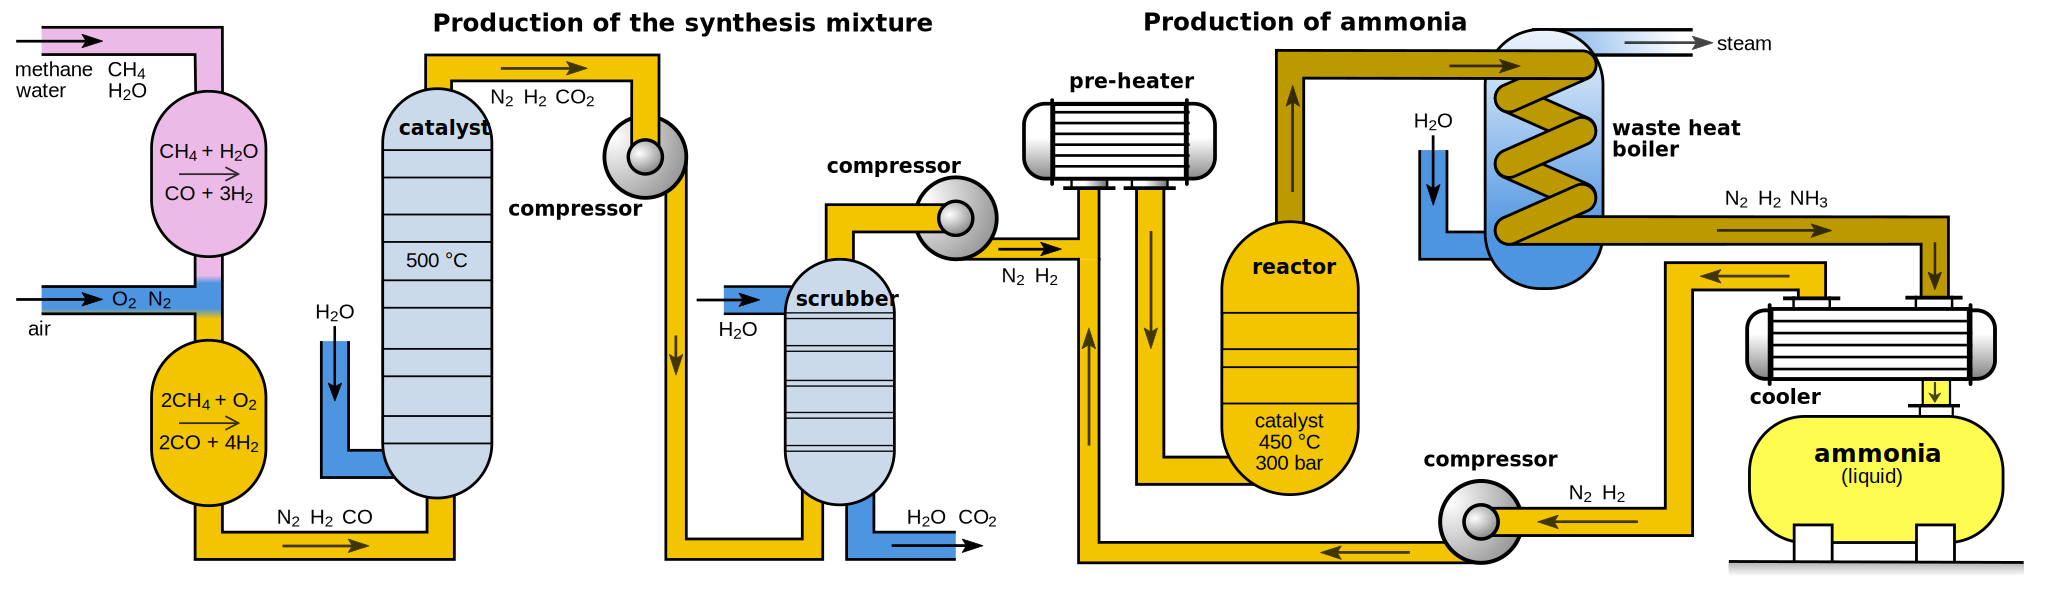
\includegraphics[width=4.4in]{images/haber-bosch-process.png}
\caption*{ %
Haber–Bosch process.\\[0.5\baselineskip]
\tiny\color{gray} Author: Francis E Williams\\
License: CC BY-SA 4.0\\
https://creativecommons.org/licenses/by-sa/4.0
}
\end{figure}

\end{frame}


%------------------------------------------%
% Consequences of Nitrogen fertilizers
%------------------------------------------%

\begin{frame}{Fertilizers in the Ecosystem}

\begin{minipage}{0.45\textwidth}

\footnotesize

\vspace{-0.5\baselineskip}

{\bfseries Benefit} -- An estimated 30 to 50\% of crop yields are attributed to natural or synthetic fertilizers.

\vspace{1\baselineskip}

{\bfseries Benefit} -- Perhaps the reason that the global population could increase from 1.6 billion in 1900 to 7.7 billion by November 2018.

\vspace{1\baselineskip}

{\bfseries Concern} -- Nitrogen use efficiency is typically less than 50\%.

\vspace{1\baselineskip}

{\bfseries Concern} -- \underline{Runoff} from industrial use can be a concern.

\end{minipage}\hspace{0.05\textwidth}%
\begin{minipage}{0.5\textwidth}

\begin{figure}
\includegraphics[width=2.25in]{images/reactive-nitrogen-cycle.jpg}
\caption*{ %
\footnotesize Global cycling of reactive nitrogen.\\[0.5\baselineskip]
\tiny\color{gray} Author: M maraviglia\\
License: CC BY-SA 4.0\\
https://creativecommons.org/licenses/by-sa/4.0
}
\end{figure}

\end{minipage}

\end{frame}

%------------------------------------------%
% Risks of fertilizers
%------------------------------------------%

\begin{frame}{Risks of Fertilizers}

\begin{figure}
\includegraphics[width=1.9in]{images/runoff.jpg}
\caption*{%
\footnotesize Runoff at a farm in Iowa.\\
{\tiny Author: Lynn Betts, U.S. Department of Agriculture}\\
}
\end{figure}

\vspace{-0.5\baselineskip}

\begin{itemize}
\footnotesize
\item Steel industry wastes may be recycled into fertilizers for their high levels of zinc (essential to plant growth) and can include the following \underline{toxic metals}:
\vspace{0.25\baselineskip}
\begin{itemize}
\footnotesize
\item Lead
\vspace{0.25\baselineskip}
\item Arsenic
\vspace{0.25\baselineskip}
\item Cadmium
\vspace{0.25\baselineskip}
\item Chromium
\end{itemize}

\end{itemize}

\end{frame}


%------------------------------------------%
% Data of the costs of cannabis cultivation
%------------------------------------------%


\begin{frame}{Data of the costs of cannabis cultivation}

\begin{minipage}{0.5\textwidth}
\begin{figure}
\includegraphics[width=\textwidth]{images/google-earth-clearing.jpg}
\end{figure}
\end{minipage}%
\begin{minipage}{0.5\textwidth}
\begin{figure}
\includegraphics[width=\textwidth]{images/google-earth-lumber.jpg}
\end{figure}
\end{minipage}

\end{frame} 


%------------------------------------------%
% Question of the day
%------------------------------------------%

%\begin{frame}{Question of the day}
%
%\begin{center}
%\begin{minipage}{\linewidth}
%\begin{Block}{Question of the Day}
%
%\vspace{0.5\baselineskip}
%
%\begin{itemize}
%
%\item 
%
%\vspace{1.5\baselineskip}
%
%\end{itemize}
%
%\end{Block}
%\end{minipage}
%\end{center}
%
%\vfill
%
%\end{minipage}
%\end{center}
%
%\end{frame}

%------------------------------------------%
% Takeaway
%------------------------------------------%
\section{Takeaway}
\begin{frame}{}

\vspace{0.5\baselineskip}

\begin{center}
\begin{minipage}{3.85in}

% Thank you.
\includegraphics[width=.25in]{images/prayer.png} {\Large \textbf{Thank you for coming.}}\\[-0.75\baselineskip]

\begin{center}
\begin{minipage}{\linewidth}
\begin{Block}{Insight of the Day}

\vspace{0.5\baselineskip}

\begin{itemize}

\item Follow the money. 
\includegraphics[scale=0.375]{images/money.pdf}

\vspace{1.5\baselineskip}

\end{itemize}

\end{Block}
\end{minipage}
\end{center}

\vfill

\end{minipage}
\end{center}

\vspace{0.5\baselineskip}

{\large What is on your mind for next week?}\\

\end{frame}


%------------------------------------------%
% Fin.
%------------------------------------------%
\end{document}
